\documentclass[a4paper,11pt]{jsarticle} % ceostyを用いるための文書クラス

% 冊子形式にするには表紙(ページ数に含まれない)で
% 1ページ使っているので最後のページのページ番号が
% 4n  ->透かしがしにくい(表紙と裏表紙の裏面が白紙)
% 4n+1->一番微妙
% 4n+2->表紙と白紙の裏表紙ができる---こうなるように調整
% 4n+3->裏表紙も使う

\usepackage{fancyhdr}	% ページスタイル

%%スタイル
% 数式やテキストの描画
\usepackage{amsmath, amsfonts, amssymb, mathtools, mathrsfs, latexsym}	% ams関連は数式書くのに必須!!
%\DeclarePairedDelimiter{\abs}{\lvert}{\rvert}
\usepackage{nccmath, empheq}	% 結構ピンポイントなパッケージ

% 画像
%% 枠だけ表示(Cannot determine size of graphicと結構怒られる)
%\usepackage[draft]{graphicx}
%% 普通に表示させる(ただ重くなりやすい)
\usepackage[dvipdfmx]{graphicx}
\usepackage[dvipdfmx]{color}
\usepackage{here}	% 絶対Hereって勝手に呼んでるやつ
\usepackage{wrapfig}	% 回り込み(ceostyのymawarikomiもある)
\usepackage{subcaption}	% minipageを使って図を並べるときの各画像のキャプションに必要

% このファイルの肝.
% usepackageの順番(ceoとの前後関係)を変えると途端にエラーを吐くので注意
%\usepackage{ceo}
% 以下のパッケージはceostyの煽りをくらったもの
\usepackage{enumerate, comment}	% 順に文書モードでの段落環境, 複数行コメント

\pagestyle{fancy}
  \lhead{2023年10月21日}
  \rhead{第2問}
  \cfoot{\thepage}

\newcommand{\vevenspace}{\vspace{\stretch{1}}}	
\newcommand{\hruleline}{\par\noindent\hrulefill\par}
\newcommand{\length}[1]{$\overline{\textup{#1}}$}
\renewcommand{\eq}{$=$}
\newcommand{\vreidai}{\vspace{\stretch{0.3}}}
\newcommand{\nn}{$n$}
\newcommand{\m}{$m$}
\newcommand{\kmath}{$k$}
\renewcommand{\O}{\textup{O}}
\newcommand{\Pn}[2]{$\textup{#1}_{#2}$}
\newcommand{\mathPn}[2]{\textup{#1}_{#2}}
\renewcommand{\P}{\textup{P}}
\newcommand{\Q}{\textup{Q}}
\newcommand{\R}{\textup{R}}
\newcommand{\A}{\textup{A}}
\newcommand{\B}{\textup{B}}
\newcommand{\C}{\textup{C}}
\newcommand{\D}{\textup{D}}
\newcommand{\numseq}[2]{$\{#1_{#2}\}$}
\newcommand{\combi}[2]{{}_{#1}\mathrm{C}_{#2}}
\newcommand{\xy}{$xy$}
\newcommand{\yz}{$yz$}
\newcommand{\xz}{$xz$}
\newcommand{\zx}{$zx$}
\newcommand{\xyz}{$xyz$}
\newcommand{\x}{$x$}
\newcommand{\y}{$y$}
\newcommand{\z}{$z$}
\newcommand{\g}{$g$}

\newcounter{numEq}
\newcommand{\assignNumEq}{%
\stepcounter{numEq}
\tag*{$\cdots\cdots$\ctext{\the\value{numEq}}}
}
\newcommand{\ctext}[1]{\raise0.2ex\hbox{\textcircled{\scriptsize{#1}}}}

%%%%%%%%%% メイン %%%%%%%%%%%
\begin{document}
%!TEX root = *.tex
%%%%%%%%%%%%%%%%%%
% カウンタのリセット
% 問題文
{
\begin{wrapfigure}{r}{14zw}
  \vspace*{-\intextsep}
  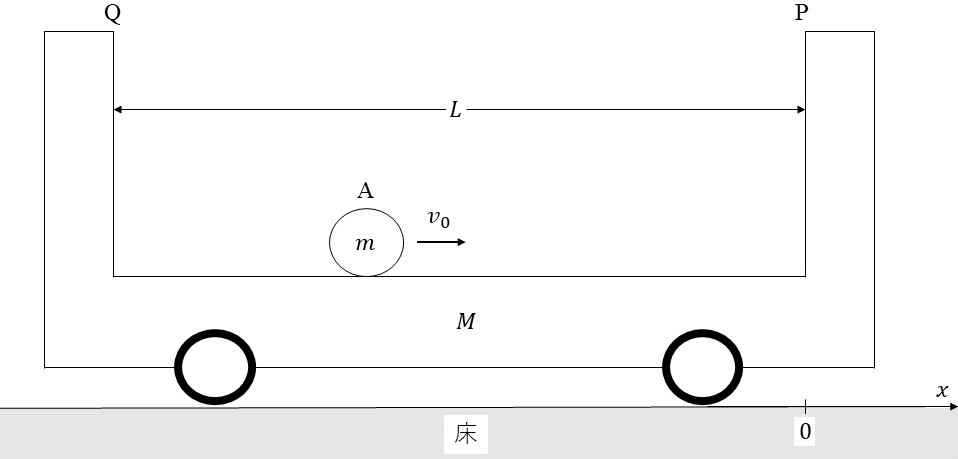
\includegraphics[width=14zw]{../graphs/jumon_42.jpg}
\end{wrapfigure}

図1のように水平な床の上に質量$M$,長さ$L$の台車が静止している.
台車の上には大きさが無視できる質量$m$の小球Aが乗っており,速度$v_0\,(v_0>0)$で運動している.
この問いで使用する速度はすべて床に対する速度であり,麦向きを正とする.
また,摩擦や空気抵抗は無視できるものとする.
\par}

\begin{enumerate}[(1)]
  \setlength{\leftskip}{-1.5zw}
  \setlength{\itemindent}{1zw}\setlength{\labelsep}{0.5zw}
  \setlength{\labelwidth}{1zw}\setlength{\leftmargin}{1zw}
  \setlength{\itemsep}{0.5\baselineskip}
  \item 小球Aが台車両端の壁P,Qに弾性衝突する場合,次の問いに答えよ.
  \begin{enumerate}[(a)]
    \setlength{\leftskip}{-2.5zw}
    \setlength{\itemindent}{1zw}\setlength{\labelsep}{1zw}
    \setlength{\labelwidth}{1zw}
    \item 小球Aが壁Pで最初に台車と衝突した直後の小球および台車の速度(それぞれ$v_1$および$V_1$)を求めよ.
    \item 小球Aは,壁Pで最初に台車と衝突してから時間$T$が経過した後に,壁Qで再び台車と衝突した.このときの時間$T$を求めよ.さらに,壁Qに衝突した直後の小球および台車の速度(それぞれ$v_2$および$V_2$)を求めよ.
    \item $M=m$の場合,小球Aと壁Pの位置の時間変化を$x\mathchar`-t$グラフに実線と点線で示せ.
    ただし,位置は床に固定された座標\x で表し,小球Aが壁Pに最初に衝突した時刻を$t=0$,位置を$x=0$として,$0\leqq t\leqq 3T$の範囲で示せ.
    \item $M=2m$の場合,台車が3Lの距離を進むのに要する時間を求めよ.
  \end{enumerate}
  \item 小球Aが台車両端の壁P,Qに反発係数$e\,(0<e<1)$で非弾性衝突する場合,次の問いに答えよ.
  \begin{enumerate}[(a)]
    \setlength{\leftskip}{-2.5zw}
    \setlength{\itemindent}{1zw}\setlength{\labelsep}{1zw}
    \setlength{\labelwidth}{1zw}
    \item 小球Aが壁Pで最初に台車と衝突した直後の小球および台車の速度(それぞれ${v_1}^\prime$および${V_1}^\prime$)を求めよ.
    \item その後,小球Aは壁Q,Pで台車と衝突をくり返した.2つの壁で合計\nn 回衝突した後の小球および台車の速度(それぞれ${v_n}^\prime$および${V_n}^\prime$)を求めよ.
    \item 十分に時間が経過し,多数の衝突をくり返した後の小球と台車の運動の様子について説明せよ.
  \end{enumerate}
\end{enumerate}



% メモ
\begin{comment}

\end{comment}


%%%%%%%%%%%%%%%%%%

\hruleline
%!TEX root = *.tex
%%%%%%%%%%%%%%%%%%
% メモ
\begin{comment}

\end{comment}
% カウンタのリセット
\setcounter{eqNo}{0}
% 解答
\noindent {\large【解答】\par}

\noindent (1)\par 
\noindent\,(a)\,
反発係数の式より
\begin{align*}
  v_0 = - (v_1-V_1) \assignEqNo
\end{align*}
運動量保存則から
\begin{align*}
  mv_0 = mv_1 + MV_1 \assignEqNo
\end{align*}
\ctext{1},\ctext{2}より
\begin{align*}
  v_1 = \dfrac{m-M}{m+M}v_0,\quad 
  V_1 = \dfrac{2m}{m+M}v_0
\end{align*}

\noindent\,(b)\,
台車に対する小球Aの速度を$u_1$とおくと
\begin{align*}
  u_1 = v_1 - V_1 = -v_0
\end{align*}
であり,台車上でPからQまでの変位$-L$を進むのに要する時間$T$は
$T=\dfrac{L}{v_0}$となる.

さらに,壁Qに衝突するときの反発係数と衝突後の運動量に注目して,
\begin{align*}
  v_1 - V_1 &= - (v_2 -V_2) \assignEqNo\\
  mv_1+MV_1 &= mv_2-MV_2 \assignEqNo
\end{align*}
\ctext{3},\ctext{4}より
\begin{align*}
  v_2 = v_0,\quad V_2 = 0
\end{align*}

{
\begin{wrapfigure}{r}{12zw}
  \vspace{-\intextsep}
  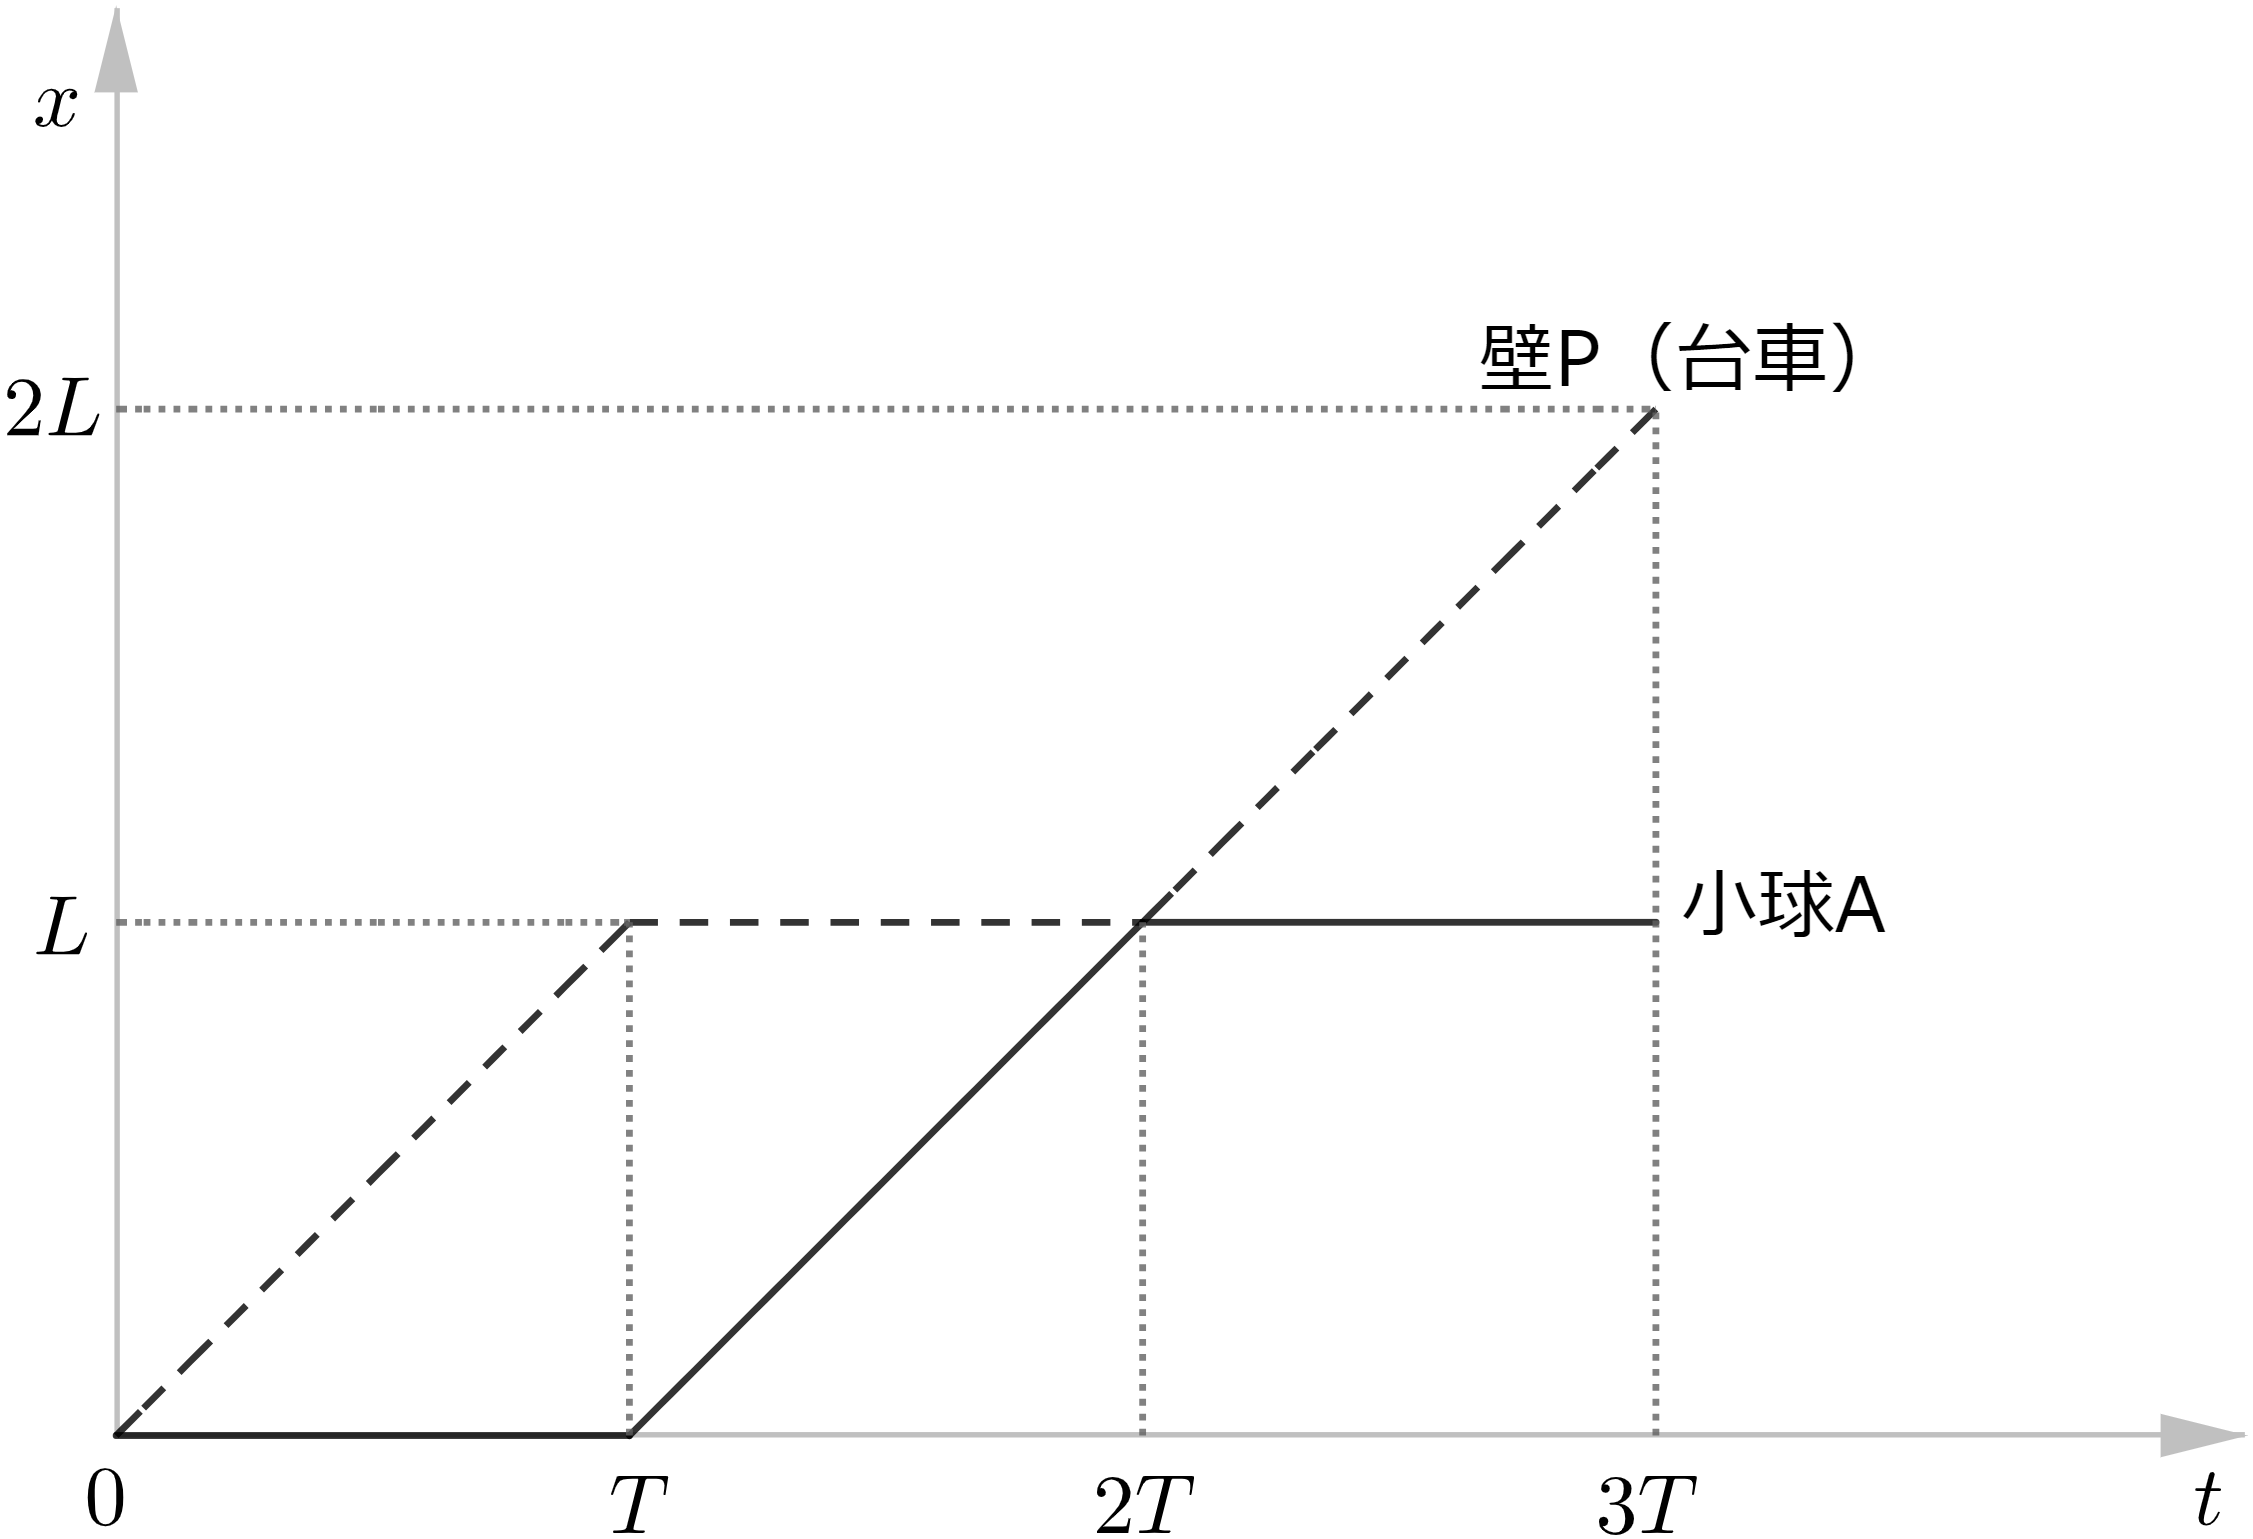
\includegraphics{../graphs/jumon_42_sol.png}
  \caption{}
\end{wrapfigure}

\noindent \,(c)\,
(2)についで,$v_3,\,V_3$を考えると,それぞれ$v_1,\,V_1$に一致する.
したがって,$m$と$M$の関係式によらず台車に対する小球Aの相対速度の大きさは$v_0$で不変であり,衝突の間隔は$T$で一定である.
いま,$m=M$より$v_1=0,\,V_1=v_0$となるので,衝突の度に速度を交換する.
すなわち,小球Aと壁Pの位置の時間変化を$x\mathchar`-t$グラフに表して,図1(右図)を得る.
\par }



\noindent \,(d)\,
$M=2m$とすると
\begin{align*}
  v_1 = -\dfrac{1}{3}v_0,\quad V_1 = \dfrac{2}{3}v_0
\end{align*}
である.
小球AがPで衝突してからQで衝突した後に再びPで衝突するまでの時刻は$2T$であり,
その間に台車が進む距離は
\begin{align*}
  \dfrac{2}{3}v_0 \cdot T = \dfrac{2}{3}L
\end{align*}
である.
また,小球がPQ間を4往復するまでに時間は$8T$かかり,その間に台車は$\dfrac{8}{3}L$進んでいる.
残り$\dfrac{1}{3}L$動くまでの時刻は$\dfrac{(1/3)L}{(2/3)v_0}=\dfrac{1}{2}T$となるので,求める時間は
\begin{align*}
  8T+T=\dfrac{17L}{2v_0}
\end{align*}
である.

\noindent (2)\par 
\noindent\,(a)\,
反発係数の式および運動量保存則より
\begin{align*}
  ev_0 &= -({v_1^\prime}-{V_1}^\prime) \assignEqNo \\
  mv_0 &= m{v_1}^\prime + M{V_1}^\prime \assignEqNo 
\end{align*}
\ctext{5},\ctext{6}より
\begin{align*}
  {v_1}^\prime = \dfrac{m-eM}{m+M}v_0,\quad 
  {V_1}^\prime = \dfrac{(1+e)M}{m+M}v_0
\end{align*}

\noindent\,(b)\,
衝突によって運動量が変わることはないので,
\begin{align*}
  mv_0 = m{v_1}^\prime + M{V_1}^\prime = \cdots = m{v_n}^\prime + M{V_n}^\prime \assignEqNo 
\end{align*}
また,各衝突における反発係数の式は
\begin{align*}
  e=-\dfrac{{v_1}^\prime-{V_1}^\prime}{v_0},\,
  e&=-\dfrac{{v_2}^\prime-{V_2}^\prime}{{v_1}^\prime-{V_1}^\prime},\,
  \cdots ,\, 
  e=-\dfrac{{v_n}^\prime-{V_n}^\prime}{{v_{n-1}}^\prime - {V_{n-1}}^\prime}
  \intertext{これらの辺々をかけ合わせて}
  (-e)^n &= \dfrac{{v_n}^\prime-{V_n}^\prime}{v_0} \assignEqNo
\end{align*}
\ctext{7},\ctext{8}より
\begin{align*}
  {v_n}^\prime = \dfrac{m+(-e)^nM}{m+M}v_0,\quad 
  {V_n}^\prime = \dfrac{\big(1-(-e)^n\big)m}{m+M}v_0
\end{align*}

\noindent\,(c)\, 
$0<e<1$ゆえ$\lim\limits_{n\to\infty}(-e)^n=0$.したがって,
\begin{align*}
  \lim_{n\to\infty}{v_n}^\prime = \dfrac{m}{m+M}v_0,\quad 
  \lim_{n\to\infty}{V_n}^\prime = \dfrac{m}{m+M}v_0
\end{align*}
以上より,十分時間の経過後,
\begin{enumerate}
  \setlength{\leftskip}{0zw}	\setlength{\itemindent}{1zw}
  \setlength{\itemsep}{0.5\baselineskip}
  \setlength{\labelwidth}{0zw}	\setlength{\labelsep}{1zw}
  \item[] 小球は台車と一体となり,速度$\dfrac{m}{m+M}v_0$の等速直線運動を行う.
\end{enumerate}


%%%%%%%%%%%%%%%%%%

\end{document}